\section{Résultats}

\paragraph*{Rendement théorique}
L'estimation de la température \(T_2\) est possible en regardant la couleur du fil chauffant. Celui-ci est observé comme étant rouge-orange ce qui correspond à une température (\(T_2 = 1143 \pm 70\)) \si{\kelvin} \cite{temp-fil}. Ainsi à l'aide de l'\autoref{eq:rend-theorie} et de la mesure de (\(T_1 = 295.0 \pm 0.1\)) \si{\kelvin} il est possible de calculer que (\(\eta_{theorie} = 74 \pm2\))\%.




\paragraph*{Caractéristiques couple-régime et rendement-régime}
Les mesures prises en éloignant le disque de freinage de l'arbre de rotation permettent d'obtenir les diagrammes reliant la vitesse angulaire au couple en \autoref{fig:couple-regime} et au rendement en \autoref{fig:rend-regime}. TODO: autoref les équations pour le couple C et le rendement eta

\begin{figure}[h]
    \centering
    \begin{subfigure}{0.5\linewidth}
        \centering
        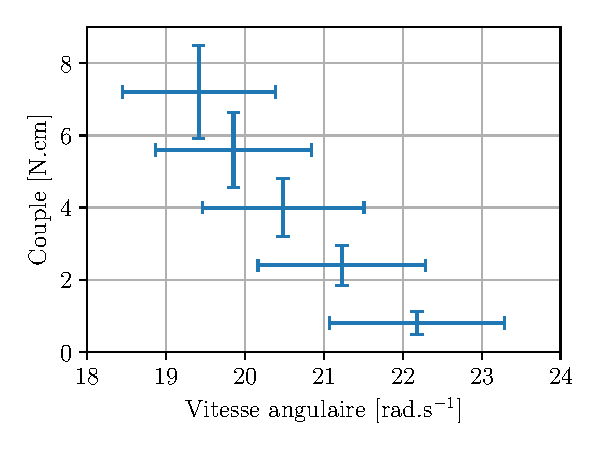
\includegraphics[width=\linewidth]{figures/couple-regime.pdf}
        \caption{}
        \label{fig:couple-regime}
    \end{subfigure}%
    \begin{subfigure}{0.5\linewidth}
        \centering
        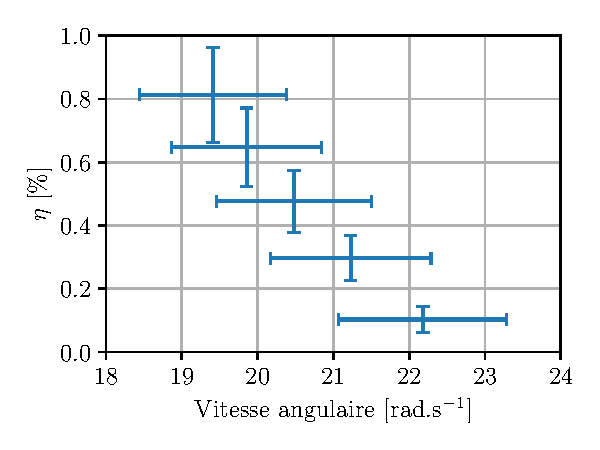
\includegraphics[width=\linewidth]{figures/rendement-regime.pdf}
        \caption{}
        \label{fig:rend-regime}
    \end{subfigure}
    \caption{Diagrammes (a) couple-régime et (b) rendement-régime}
\end{figure}



\begin{minipage}{\linewidth}
    \begin{wrapfigure}{R}{0.5\linewidth}
        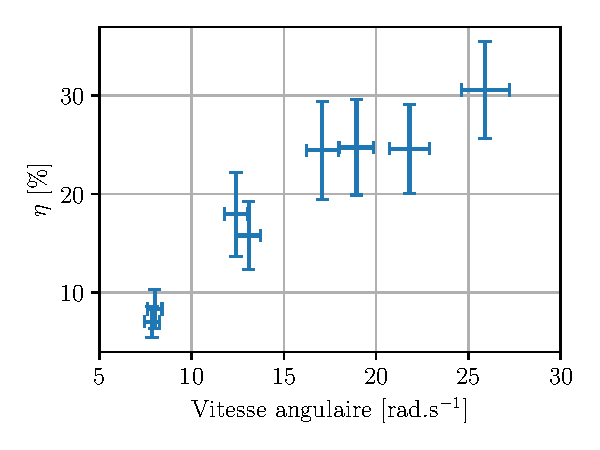
\includegraphics[width=\linewidth]{figures/rend-frigo.pdf}
        \caption{Rendement du cycle frigorifique en fonction du régime de l'arbre de rotation}
        \label{fig:rend-frigo}
    \end{wrapfigure}

    \paragraph*{Rendement du cycle frigorifique}
    Les mesures des puissances fournies au moteur et au filament de compensation permettent un calcul du rendement par l'\autoref{eq:rend-frigo}. La valeur de la température d'équilibre du système entre le refroidissement et la compensation n'a pas été exactement constante sur l'ensemble des mesures mais a tout de même variée de moins de 10 \si{\kelvin}. Les rendements obtenus sont représentés avec leurs barres d'erreur sur la vitesse angulaire et sur le rendement en \autoref{fig:rend-frigo}.

\end{minipage}


